\documentclass[14pt]{extarticle}
\usepackage{fontspec}
\usepackage{polyglossia}
\usepackage{amsmath}
\usepackage{amssymb}
\usepackage{xcolor}
\usepackage{fancyhdr}
\usepackage{graphicx}
\usepackage{listings}
\usepackage[most]{tcolorbox}
% \usepackage{setspace}
\usepackage{pifont}
\usepackage{enumitem}
\usepackage{titlesec}
\usepackage[bottom]{footmisc}
\usepackage{titling}
\usepackage{minted}
\usepackage{etoolbox}
\usepackage{array}
\usepackage{extsizes}
\usepackage{float}
\usepackage{booktabs}
\usepackage{hyperref}
\usepackage[onehalfspacing]{setspace}
\usepackage[a4paper, top=2.7cm, bottom=2.7cm, left=2.5cm, right=2.5cm, headheight=1.5cm, headsep=0.5cm]{geometry}
\usepackage{tikz}

\usetikzlibrary{automata, positioning, arrows.meta, arrows}

\newfontfamily\emoji{Segoe UI Emoji}

\pagestyle{fancy}

\setmainlanguage[numerals=western]{arabic}
\setotherlanguage{english}
% \newfontfamily\arabicfont[Script=Arabic]{Amiri}
\newfontfamily\arabicfont[Script=Arabic]{Calibri}
\newfontfamily\arabicfonttt[Script=Arabic]{Courier New}

\lstset{
  language=[Sharp]C,
  numbers=left,
  stepnumber=1,
  numbersep=8pt,
  frame=single,
  basicstyle=\ttfamily\small,
  keywordstyle=\color{blue},
  stringstyle=\color{red},
  commentstyle=\color{green!50!black}
}

\newif\ifdetailed
\ifdefined\setdetailed
  \setdetailed
\fi

\newif\ifwithsols
\ifdefined\setwithsols
  \setwithsols
\fi

% unified tcolorboxes for articles
\tcbset{colback=white, colframe=black, fonttitle=\bfseries, boxrule=0.8pt}
\newtcolorbox{boxDef}[1][]{colback=blue!5!white,colframe=blue!75!black,
  title={{\emoji📘} تعريف\ifx\\#1\\\else ~#1\fi :}}
\newtcolorbox{boxExercise}[1][]{colback=cyan!5!white,colframe=cyan!70!black,
  title={{\emoji🧩} تمرين\ifx\\#1\\\else ~#1\fi :}}
\newtcolorbox{boxExample}[1][]{colback=yellow!5!white,colframe=orange!90!black,
  title={{\emoji📝} مثال\ifx\\#1\\\else ~#1\fi :}}
\newtcolorbox{boxNote}[1][]{colback=gray!10!white,colframe=black,
  title={{\emoji✨} ملاحظة\ifx\\#1\\\else ~#1\fi :}}
\newtcolorbox{boxAttention}[1][]{colback=magenta!10!white,colframe=magenta!80!black,
  title={{\emoji🔔} تنبيه\ifx\\#1\\\else ~#1\fi :}}
\newtcolorbox{boxWarning}[1][]{colback=red!5!white,colframe=red!75!black,
  title={{\emoji⚡} ملاحظة هامة\ifx\\#1\\\else ~#1\fi :}}
\newtcolorbox{boxSolution}[1][]{colback=green!5!white,colframe=green!60!black,
  title={{\emoji✅} حل\ifx\\#1\\\else ~#1\fi :}}
\newtcolorbox{boxSymbol}[1][]{colback=purple!5!white,colframe=purple!70!black,
  title={{\emoji🔣} رمز\ifx\\#1\\\else ~#1\fi :}}
\newtcolorbox{boxHint}[1][]{colback=teal!5!white,colframe=teal!60!black,
  title={{\emoji💡} تلميح\ifx\\#1\\\else ~#1\fi :}}


\tcbset{simplecode/.style={ colback=gray!5, colframe=black!50, boxrule=0.4pt, arc=2pt, left=4pt,right=4pt,top=4pt,bottom=4pt}}
\newenvironment{boxCode}{\begin{tcolorbox}[simplecode]}{\end{tcolorbox}}

\newcolumntype{C}[1]{>{\centering\arraybackslash}p{#1}}

% redefine spaces after titles
\makeatletter
\renewcommand{\@maketitle}{%
  \begin{center}
    {\huge \bfseries \@title \par}%
    \vskip 0.2em % space between title and author
    {\large \@author \par}%
    % \vskip 0.2em % space between author and date
    % {\normalsize \@date \par}%
  \end{center}
}
\makeatother

\fancyhf{} % clear default
\fancypagestyle{plain}{
  \fancyhf{}
  \fancyhead[L]{مدرسة التسامح الشاملة}
  % \fancyhead[L]{
\includegraphics[height=1cm]{../../../images/logoTasamoh.png}}
  \fancyhead[R]{الأستاذ محمود اغبارية}
  \fancyfoot[C]{\thepage}
}

\fancyhead[L]{مدرسة التسامح الشاملة}
\fancyhead[R]{الأستاذ محمود اغبارية}
\fancyfoot[C]{\thepage}
% \date{\today}

\setcounter{tocdepth}{3} % only section subsection and subsubsection in TOC

\newcommand{\importpdfpage}[2]{%
    \thispagestyle{empty}
    \newgeometry{left=0cm,right=0cm,top=0cm,bottom=0cm}
    \includegraphics[page=#2,width=0.95\paperwidth,height=0.95\paperheight,keepaspectratio]{#1}
    \restoregeometry
}

\newcommand{\insertFullImg}[1]{%
    \noindent
    \makebox[\textwidth][c]{
        \includegraphics[width=0.9\paperwidth,keepaspectratio]{#1}%
    }%
}%

% ----------------------


% \begin{document}

% \maketitle

% % \clearpage  % start TOC on a new page
% % \renewcommand{\contentsname}{جدول المحتويات}
% % \tableofcontents
% % \clearpage

% \part*{part 1} % the * prevents numbering
% \section*{مقدمة}
% \subsection*{مثال رياضي}
% \subsubsection*{مثال فرعي}
% \paragraph*{ paragraph 1}
% \subparagraph*{sub paragraph 1}

% \ifdetailed
% \begin{english}
% \begin{minted}{csharp}
% // C# Example
% \end{minted}
% \end{english}
% \fi

% OLD WAY
% \ifdetailed
% \begin{english}
% \begin{lstlisting}
% // C# Example
% \end{lstlisting}
% \end{english}
% \fi

% % 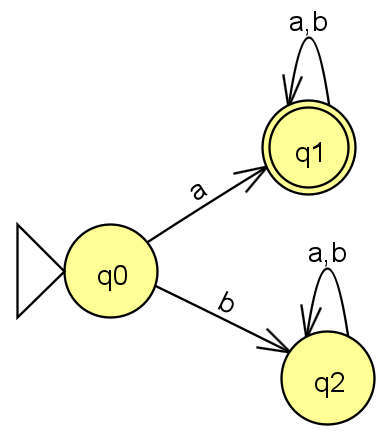
\includegraphics[width=0.2\textwidth]{../../../images/DFAs/ex1_q1.png}



% \vspace{3cm}
% \begin{flushleft}
% أرجو لكم وقتًا ممتعًا.

% الأستاذ محمود اغبارية.
% \end{flushleft}


% \end{document}


\ifwithsols
\title{حل ورقة تمرّن 17: الفئات والكائنات 2}
\else
\title{ورقة تمرّن 17: الفئات والكائنات 2}
\fi

\begin{document}

\maketitle
\thispagestyle{fancy}

% ======================================================
% سؤال 1 - فئة Student
% ======================================================
\begin{enumerate}[itemsep=2em]

\item
سنبني فئة تمثل طالبًا في المدرسة.
\begin{enumerate}[itemsep=1em]
    \item أنشئ فئة باسم \textenglish{Student} تحتوي على الحقول الخاصة (\textenglish{private}) التالية:
    \begin{itemize}[itemsep=1pt]
        \item \textenglish{string Name} — اسم الطالب
        \item \textenglish{int Grade} — الصف (من 1 إلى 12)
        \item \textenglish{double Average} — معدل الطالب (من 0 إلى 100)
    \end{itemize}
    أضف عملية بنّاءة تستقبل الاسم والصف والمعدل وتهيئ الحقول.

    \item أضف عمليات الاسترجاع (\textenglish{Getters}):
    \textenglish{GetName()}, \textenglish{GetGrade()}, \textenglish{GetAverage()}.

    \item أضف عملية \textenglish{SetAverage(double newAverage)} تُعدِّل المعدل فقط إذا كانت القيمة بين \textenglish{0} و \textenglish{100}.

    \item أضف عملية \textenglish{void Print()} تطبع بيانات الطالب بالتنسيق التالي: \\
    \textenglish{Name: Sara | Grade: 10 | Average: 91.5}

    \item أضف عملية \textenglish{bool IsPassing()} تعيد \textenglish{true} إذا كان المعدل أكبر من أو يساوي \textenglish{55.0}.

    \item أضف عملية \textenglish{bool HasHigherAverageThan(Student other)} تعيد \textenglish{true} إذا كان معدل الكائن الحالي أعلى من معدل الطالب \textenglish{other}.\\
    تحقق من \textenglish{null} قبل الاستخدام.

    \item في الدالة الرئيسية \textenglish{Main}، قُم بكتابة الأوامر التالية بالترتيب لاختبار الفئة:
    \begin{itemize}[itemsep=1pt]
        \item عرّف كائنًا جديدًا يمثل طالبًا، ومرر للبنّاء القيم: \textenglish{"Sara"}، \textenglish{10}، \textenglish{91.5}.
        \item عرّف كائنًا ثانيًا، ومرر للبنّاء القيم: \textenglish{"Khalil"}، \textenglish{11}، \textenglish{85.0}.
        \item استدعِ الدالة \textenglish{Print()} لكل من الكائنين لطباعة بياناتهما الأولية.
        \item استدعِ الدالة \textenglish{SetAverage} لتعديل معدل الطالب الثاني (\textenglish{"Khalil"}) ليصبح \textenglish{52.0}.
        \item اطبع عبارة توضيحية على الشاشة مع استدعاء الدالة \textenglish{IsPassing()} للطالب الثاني للتحقق من حالة نجاحه بعد التعديل.
    \end{itemize}
\end{enumerate}

\ifwithsols
{\small
\begin{boxSolution}
\begin{english}
\begin{minted}{csharp}
class Student
{
    private string Name;
    private int Grade;
    private double Average;

    public Student(string name, int grade, double average)
    {
        this.Name    = name;
        this.Grade   = grade;
        this.Average = average;
    }

    public string GetName()    { return Name;    }
    public int    GetGrade()   { return Grade;   }
    public double GetAverage() { return Average; }

    public void SetAverage(double newAverage)
    {
        if (newAverage >= 0 && newAverage <= 100)
            Average = newAverage;
    }

    public void Print()
    {
        Console.WriteLine($"Name: {Name} | Grade: {Grade} | Average: {Average}");
    }

    public bool IsPassing()
    {
        return Average >= 55.0;
    }

    public bool HasHigherAverageThan(Student other)
    {
        if (other == null)
            return false;
        return this.Average > other.Average;
    }
}
\end{minted}
\end{english}
\end{boxSolution}
\begin{boxSolution}
\begin{english}
\begin{minted}{csharp}
// In Main
Student s1 = new Student("Sara", 10, 91.5);
Student s2 = new Student("Khalil", 11, 85.0);

s1.Print();
s2.Print();

s2.SetAverage(52.0);
Console.WriteLine("Is Khalil passing? " + s2.IsPassing());
\end{minted}
\end{english}
\end{boxSolution}
}
\fi
\clearpage

% ======================================================
% سؤال 2 - فئة Movie
% ======================================================
\item
سنبني فئة تمثل فيلمًا سينمائيًا.
\begin{enumerate}[itemsep=1em]
    \item أنشئ فئة باسم \textenglish{Movie} تحتوي على الحقول الخاصة (\textenglish{private}) التالية:
    \begin{itemize}[itemsep=1pt]
        \item \textenglish{string Title} — عنوان الفيلم
        \item \textenglish{string Director} — اسم المخرج
        \item \textenglish{int Year} — سنة الإنتاج
        \item \textenglish{double Rating} — التقييم (من 0.0 إلى 10.0)
    \end{itemize}

    \item أضف عملية بنّاءة تستقبل العنوان والمخرج والسنة والتقييم وتهيئ الحقول.

    \item أضف عمليات الاسترجاع (\textenglish{Getters}) للحقول الأربعة.

    \item أضف عملية \textenglish{SetRating(double newRating)} تُعدِّل التقييم فقط إذا كانت القيمة بين \textenglish{0.0} و \textenglish{10.0}.

    \item أضف عملية \textenglish{bool IsHighlyRated()} تعيد \textenglish{true} إذا كان التقييم أكبر من أو يساوي \textenglish{8.0}.

    \item أضف عملية \textenglish{void Print()} تطبع الفيلم بالتنسيق التالي: \\
    \textenglish{"Inception" by Nolan (2010) - Rating: 9.3}

    \item في الدالة الرئيسية \textenglish{Main}، قُم بكتابة الأوامر التالية بالترتيب لاختبار الفئة:
    \begin{itemize}[itemsep=1pt]
        \item عرّف كائنًا يمثل فيلم \textenglish{"Inception"} للمخرج \textenglish{"Nolan"}، إنتاج عام \textenglish{2010}، وبتقييم \textenglish{9.3}.
        \item عرّف كائنًا ثانيًا يمثل فيلم \textenglish{"The Room"} للمخرج \textenglish{"Wiseau"}، إنتاج عام \textenglish{2003}، وبتقييم \textenglish{3.7}.
        \item استدعِ الدالة \textenglish{Print()} لكل فيلم لطباعة تفاصيله على الشاشة.
        \item استخدم الدالة \textenglish{SetRating} لتخفيض تقييم الفيلم الأول (\textenglish{"Inception"}) ليصبح \textenglish{7.5}.
        \item اطبع عبارة توضيحية مع استدعاء الدالة \textenglish{IsHighlyRated()} للفيلم الأول للتحقق مما إذا كان لا يزال يعتبر ذا تقييم عالٍ (مقارنةً بالشرط).
    \end{itemize}
\end{enumerate}

\ifwithsols
{\small
\begin{boxSolution}
\begin{english}
\begin{minted}{csharp}
// a, b, c, d, e, f
class Movie
{
    private string Title;
    private string Director;
    private int Year;
    private double Rating;

    public Movie(string title, string director, int year, double rating)
    {
        this.Title    = title;
        this.Director = director;
        this.Year     = year;
        this.Rating   = rating;
    }

    public string GetTitle()    { return Title;    }
    public string GetDirector() { return Director; }
    public int    GetYear()     { return Year;     }
    public double GetRating()   { return Rating;   }

    public void SetRating(double newRating)
    {
        if (newRating >= 0.0 && newRating <= 10.0)
            Rating = newRating;
    }

    public bool IsHighlyRated()
    {
        return Rating >= 8.0;
    }

    public void Print()
    {
        Console.WriteLine($"\"{Title}\" by {Director} ({Year}) - Rating: {Rating}");
    }
}
\end{minted}
\end{english}
\end{boxSolution}
\begin{boxSolution}
\begin{english}
\begin{minted}{csharp}
// In Main:
Movie m1 = new Movie("Inception", "Nolan", 2010, 9.3);
Movie m2 = new Movie("The Room", "Wiseau", 2003, 3.7);

m1.Print();
m2.Print();

m1.SetRating(7.5);
Console.WriteLine("Is m1 highly rated? " + m1.IsHighlyRated());
\end{minted}
\end{english}
\end{boxSolution}
}
\fi
\clearpage


% ======================================================
% سؤال 4 - فئة Temperature
% ======================================================
\item
سنبني فئة تمثل قراءة درجة حرارة.
\begin{enumerate}[itemsep=1em]
    \item أنشئ فئة باسم \textenglish{Temperature} تحتوي على الحقل الخاص (\textenglish{private}) التالي:
    \begin{itemize}[itemsep=1pt]
        \item \textenglish{double Celsius} — درجة الحرارة بالسلسيوس
    \end{itemize}
    أضف عملية بنّاءة تستقبل قيمة بالسلسيوس وتهيئ الحقل.

    \item أضف عملية استرجاع \textenglish{GetCelsius()}.

    \item أضف عملية \textenglish{double ToFahrenheit()} تعيد درجة الحرارة محوّلةً إلى فهرنهايت.\\
    \textbf{القانون:} \textenglish{F = C * 9 / 5 + 32}

    \item أضف عملية \textenglish{double ToKelvin()} تعيد درجة الحرارة محوّلةً إلى كلفن.\\
    \textbf{القانون:} \textenglish{K = C + 273.15}

    \item أضف عملية \textenglish{string GetCategory()} تعيد وصفًا حسب الجدول:
    \begin{itemize}[itemsep=1pt]
        \item أقل من \textenglish{0}: \textenglish{"Freezing"}
        \item من \textenglish{0} إلى \textenglish{15}: \textenglish{"Cold"}
        \item من \textenglish{15} إلى \textenglish{30}: \textenglish{"Comfortable"}
        \item أكبر من \textenglish{30}: \textenglish{"Hot"}
    \end{itemize}

    \item أضف عملية \textenglish{bool IsWarmerThan(Temperature other)} تعيد \textenglish{true} إذا كان الكائن الحالي أدفأ من \textenglish{other}.

    \item في الدالة الرئيسية \textenglish{Main}، قُم بكتابة الأوامر التالية بالترتيب لاختبار الفئة:
    \begin{itemize}[itemsep=1pt]
        \item عرّف كائنًا أول لدرجة الحرارة بقيمة \textenglish{25.0} مئوية (سلسيوس).
        \item عرّف كائنًا ثانيًا لدرجة الحرارة بقيمة \textenglish{-5.0} مئوية.
        \item اطبع بيانات الكائن الأول بحيث تعرض: درجة الحرارة بالسلسيوس، ما يعادلها بالفهرنهايت، ما يعادلها بالكلفن، والتصنيف الخاص بها (باستدعاء الدوال المناسبة).
        \item اطبع بيانات الكائن الثاني بالطريقة نفسها.
        \item استخدم الدالة \textenglish{IsWarmerThan} للتحقق مما إذا كان الكائن الأول أدفأ من الكائن الثاني، واطبع النتيجة على الشاشة.
    \end{itemize}
\end{enumerate}

\ifwithsols
{\small
\begin{boxSolution}
\begin{english}
\begin{minted}{csharp}
class Temperature
{
    private double Celsius;

    public Temperature(double celsius)
    {
        this.Celsius = celsius;
    }

    public double GetCelsius() { return Celsius; }

    public double ToFahrenheit()
    {
        return Celsius * 9.0 / 5.0 + 32;
    }

    public double ToKelvin()
    {
        return Celsius + 273.15;
    }

    public string GetCategory()
    {
        if (Celsius < 0)
            return "Freezing";
        if (Celsius <= 15)
            return "Cold";
        if (Celsius <= 30)
            return "Comfortable";
        return "Hot";
    }

    public bool IsWarmerThan(Temperature other)
    {
        if (other == null)
            return false;
        return this.Celsius > other.Celsius;
    }
}
\end{minted}
\end{english}
\end{boxSolution}
\begin{boxSolution}
\begin{english}
\begin{minted}{csharp}
// In Main:
Temperature t1 = new Temperature(25.0);
Temperature t2 = new Temperature(-5.0);

Console.WriteLine($"t1: {t1.GetCelsius()}C = {t1.ToFahrenheit()}F = {t1.ToKelvin()}K | {t1.GetCategory()}");
Console.WriteLine($"t2: {t2.GetCelsius()}C = {t2.ToFahrenheit()}F = {t2.ToKelvin()}K | {t2.GetCategory()}");
Console.WriteLine("Is t1 warmer than t2? " + t1.IsWarmerThan(t2));
\end{minted}
\end{english}
\end{boxSolution}
}
\fi

\end{enumerate}

\vspace{1cm}
\begin{flushleft}
أرجو لكم عملاً ممتعاً!

الأستاذ محمود اغبارية.
\end{flushleft}

\end{document}